\documentclass{standalone}
\usepackage{tikz}
\usetikzlibrary{patterns}
\usetikzlibrary{positioning}
\usetikzlibrary{patterns, positioning}
\usetikzlibrary{shapes.misc}
\usepackage[outline]{contour}
\contourlength{1.5pt} 
\usepackage[sfdefault]{ClearSans}

\begin{document}
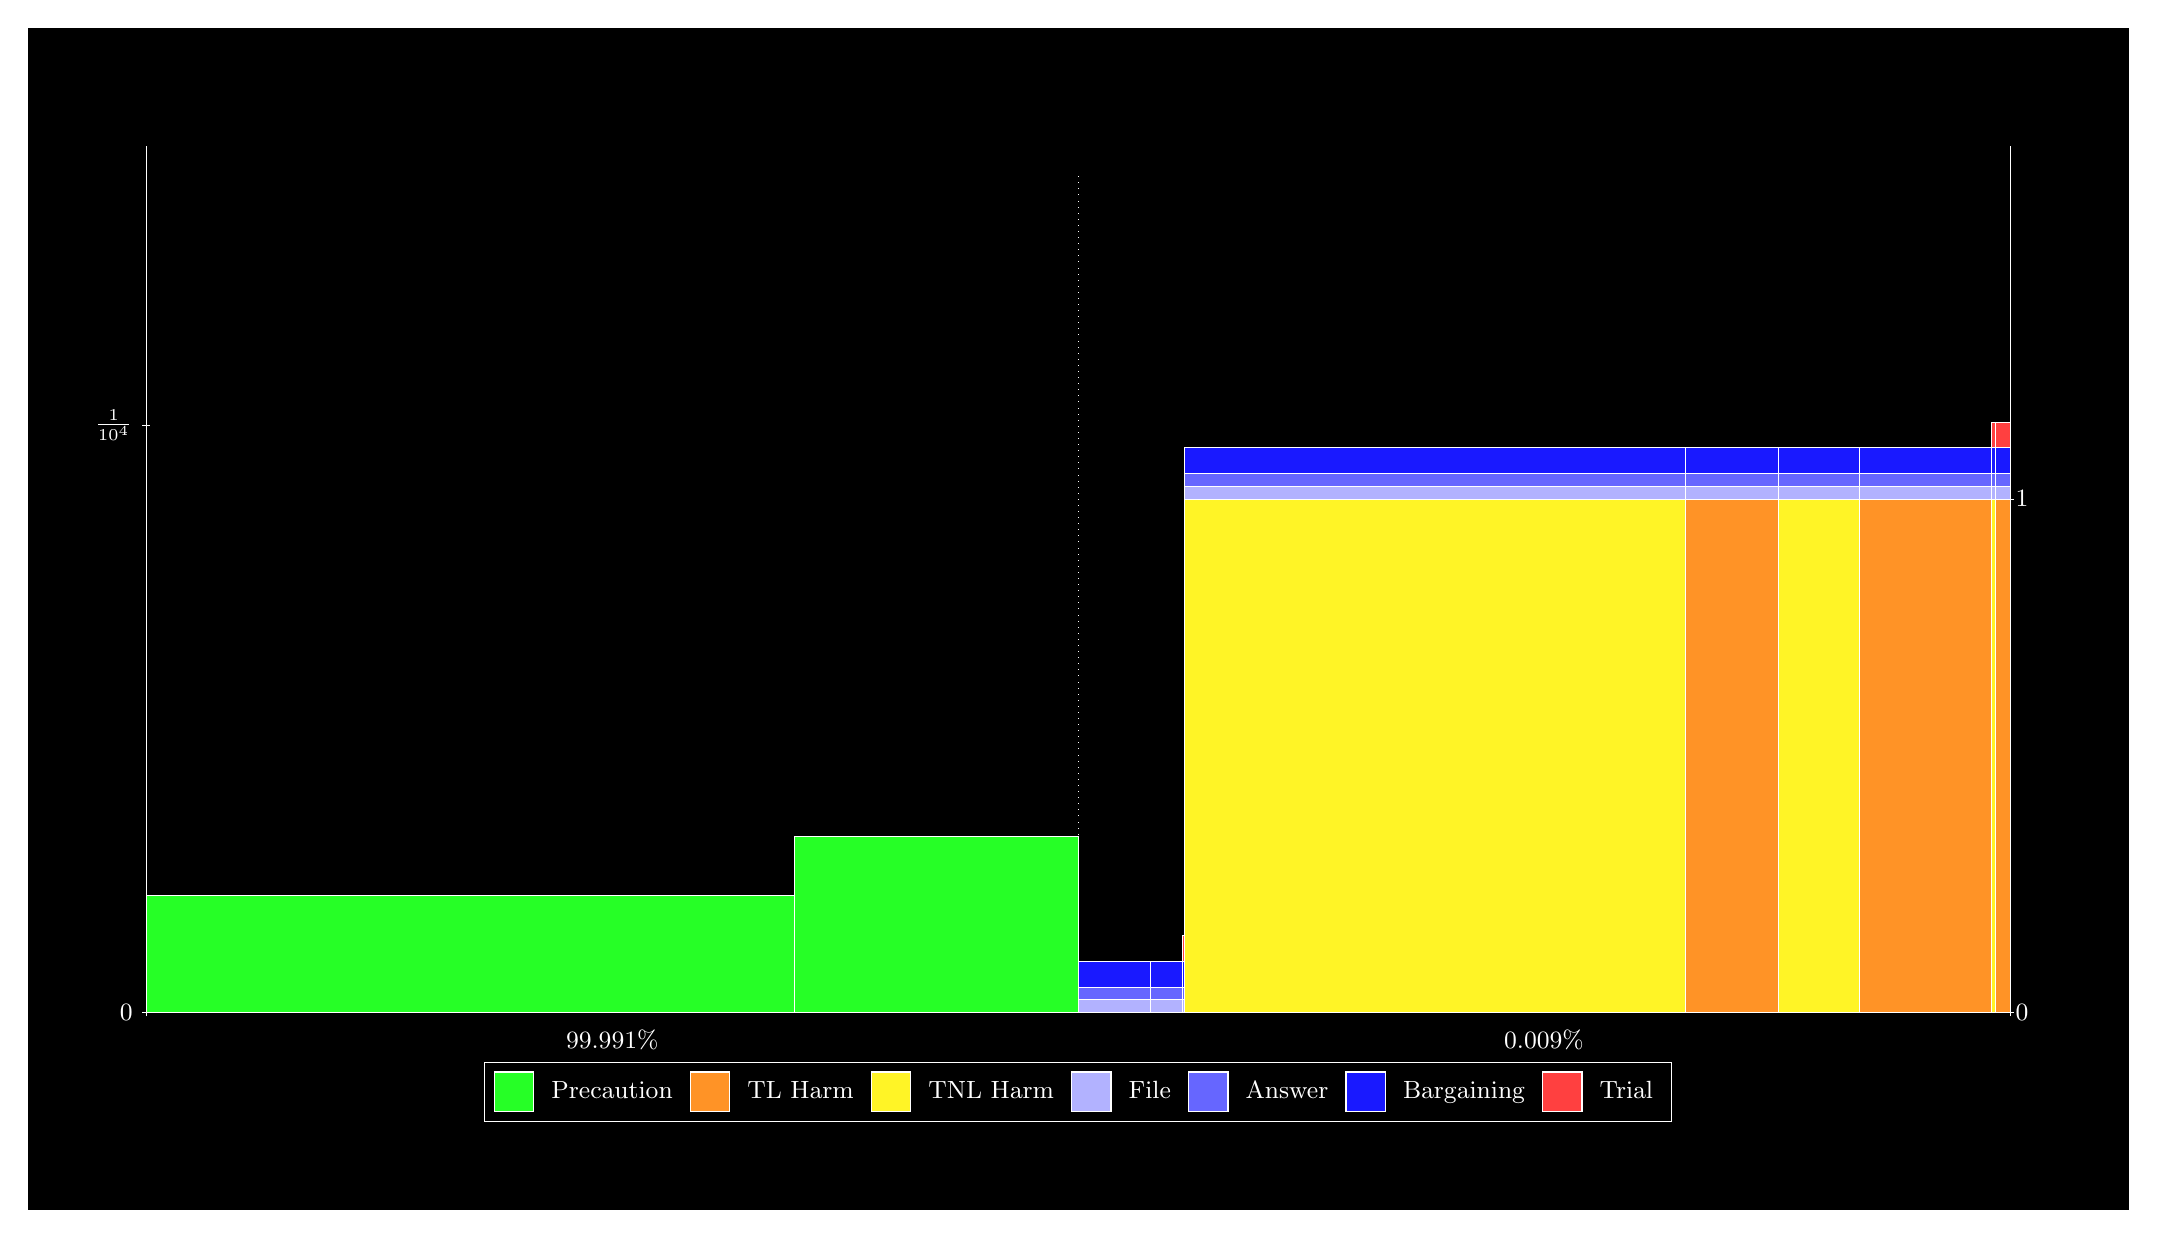
\begin{tikzpicture}
\draw[fill=black] (0,0) rectangle (26.667,15);
\draw[fill=green!85,draw=white,very thin] (1.5,2.5) rectangle (9.7243,3.9918);
\draw[fill=green!85,draw=white,very thin] (9.7243,2.5) rectangle (13.333,4.7377);
\draw[fill=green!85,draw=white,very thin] (13.333,2.5) rectangle (14.244,2.5001);
\draw[fill=blue!30,draw=white,very thin] (13.333,2.5001) rectangle (14.244,2.6632);
\draw[fill=blue!60,draw=white,very thin] (13.333,2.6632) rectangle (14.244,2.8262);
\draw[fill=blue!90,draw=white,very thin] (13.333,2.8262) rectangle (14.244,3.1523);
\draw[fill=green!85,draw=white,very thin] (14.244,2.5) rectangle (14.656,2.5002);
\draw[fill=blue!30,draw=white,very thin] (14.244,2.5002) rectangle (14.656,2.6632);
\draw[fill=blue!60,draw=white,very thin] (14.244,2.6632) rectangle (14.656,2.8263);
\draw[fill=blue!90,draw=white,very thin] (14.244,2.8263) rectangle (14.656,3.1524);
\draw[fill=green!85,draw=white,very thin] (14.656,2.5) rectangle (14.687,2.5001);
\draw[fill=blue!30,draw=white,very thin] (14.656,2.5001) rectangle (14.687,2.6632);
\draw[fill=blue!60,draw=white,very thin] (14.656,2.6632) rectangle (14.687,2.8262);
\draw[fill=blue!90,draw=white,very thin] (14.656,2.8262) rectangle (14.687,3.1523);
\draw[fill=red!75,draw=white,very thin] (14.656,3.1523) rectangle (14.687,3.4784);
\draw[fill=green!85,draw=white,very thin] (14.687,2.5) rectangle (21.047,2.5001);
\draw[fill=yellow!85,draw=white,very thin] (14.687,2.5001) rectangle (21.047,9.022);
\draw[fill=blue!30,draw=white,very thin] (14.687,9.022) rectangle (21.047,9.1851);
\draw[fill=blue!60,draw=white,very thin] (14.687,9.1851) rectangle (21.047,9.3481);
\draw[fill=blue!90,draw=white,very thin] (14.687,9.3481) rectangle (21.047,9.6742);
\draw[fill=green!85,draw=white,very thin] (21.047,2.5) rectangle (22.223,2.5001);
\draw[fill=orange!85,draw=white,very thin] (21.047,2.5001) rectangle (22.223,9.022);
\draw[fill=blue!30,draw=white,very thin] (21.047,9.022) rectangle (22.223,9.1851);
\draw[fill=blue!60,draw=white,very thin] (21.047,9.1851) rectangle (22.223,9.3481);
\draw[fill=blue!90,draw=white,very thin] (21.047,9.3481) rectangle (22.223,9.6742);
\draw[fill=green!85,draw=white,very thin] (22.223,2.5) rectangle (23.25,2.5002);
\draw[fill=yellow!85,draw=white,very thin] (22.223,2.5002) rectangle (23.25,9.0221);
\draw[fill=blue!30,draw=white,very thin] (22.223,9.0221) rectangle (23.25,9.1852);
\draw[fill=blue!60,draw=white,very thin] (22.223,9.1852) rectangle (23.25,9.3482);
\draw[fill=blue!90,draw=white,very thin] (22.223,9.3482) rectangle (23.25,9.6743);
\draw[fill=green!85,draw=white,very thin] (23.25,2.5) rectangle (24.934,2.5002);
\draw[fill=orange!85,draw=white,very thin] (23.25,2.5002) rectangle (24.934,9.0221);
\draw[fill=blue!30,draw=white,very thin] (23.25,9.0221) rectangle (24.934,9.1852);
\draw[fill=blue!60,draw=white,very thin] (23.25,9.1852) rectangle (24.934,9.3482);
\draw[fill=blue!90,draw=white,very thin] (23.25,9.3482) rectangle (24.934,9.6743);
\draw[fill=green!85,draw=white,very thin] (24.934,2.5) rectangle (24.985,2.5001);
\draw[fill=yellow!85,draw=white,very thin] (24.934,2.5001) rectangle (24.985,9.022);
\draw[fill=blue!30,draw=white,very thin] (24.934,9.022) rectangle (24.985,9.1851);
\draw[fill=blue!60,draw=white,very thin] (24.934,9.1851) rectangle (24.985,9.3481);
\draw[fill=blue!90,draw=white,very thin] (24.934,9.3481) rectangle (24.985,9.6742);
\draw[fill=red!75,draw=white,very thin] (24.934,9.6742) rectangle (24.985,10);
\draw[fill=green!85,draw=white,very thin] (24.985,2.5) rectangle (25.167,2.5001);
\draw[fill=orange!85,draw=white,very thin] (24.985,2.5001) rectangle (25.167,9.022);
\draw[fill=blue!30,draw=white,very thin] (24.985,9.022) rectangle (25.167,9.1851);
\draw[fill=blue!60,draw=white,very thin] (24.985,9.1851) rectangle (25.167,9.3481);
\draw[fill=blue!90,draw=white,very thin] (24.985,9.3481) rectangle (25.167,9.6742);
\draw[fill=red!75,draw=white,very thin] (24.985,9.6742) rectangle (25.167,10);
\draw[white,very thin] (1.5,2.5) -- (1.5,13.5);
\draw[white,very thin] (1.45,2.5) -- (1.55,2.5);
\node[font=\small,text=white, anchor=east] at (1.45, 2.5) {0};
\draw[white,very thin] (1.45,9.9591) -- (1.55,9.9591);
\node[font=\small,text=white, anchor=east] at (1.45, 9.9591) {$\frac{1}{10^{4}}$};

\draw[white,dotted,very thin] (13.333,2.83) -- (13.333,13.17);
\draw[white,very thin] (25.167,2.5) -- (25.167,13.5);
\draw[white,very thin] (25.117,2.5) -- (25.217,2.5);
\node[font=\small,text=white, anchor=west] at (25.117, 2.5) {0};
\draw[white,very thin] (25.117,9.0219) -- (25.217,9.0219);
\node[font=\small,text=white, anchor=west] at (25.117, 9.0219) {1};

\draw[white,very thin] (1.5,2.5) -- (25.167,2.5);
\draw[white,very thin] (1.5,2.45) -- (1.5,2.55);
\node[font=\small,text=white, anchor=north] at (1.5, 2.45) {};
\draw[white,very thin] (25.167,2.45) -- (25.167,2.55);
\node[font=\small,text=white, anchor=north] at (25.167, 2.45) {};

\node[font=\small,text=white,anchor=south] at (7.4167, 1.9) {99.991\%};
\node[font=\small,text=white,anchor=south] at (19.25, 1.9) {0.009\%};
\draw (13.3333,2.5) node (B) {};
\begin{scope}[align=center]
\matrix[scale=0.5,draw=white,below=0.5cm of B,nodes={draw},column sep=0.1cm]{
\node[rectangle,draw,minimum width=0.5cm,minimum height=0.5cm,fill=green!85]{}; & \node[draw=none,font=\small,text=white]{Precaution}; &
\node[rectangle,draw,minimum width=0.5cm,minimum height=0.5cm,fill=orange!85]{}; & \node[draw=none,font=\small,text=white]{TL Harm}; &
\node[rectangle,draw,minimum width=0.5cm,minimum height=0.5cm,fill=yellow!85]{}; & \node[draw=none,font=\small,text=white]{TNL Harm}; &
\node[rectangle,draw,minimum width=0.5cm,minimum height=0.5cm,fill=blue!30]{}; & \node[draw=none,font=\small,text=white]{File}; &
\node[rectangle,draw,minimum width=0.5cm,minimum height=0.5cm,fill=blue!60]{}; & \node[draw=none,font=\small,text=white]{Answer}; &
\node[rectangle,draw,minimum width=0.5cm,minimum height=0.5cm,fill=blue!90]{}; & \node[draw=none,font=\small,text=white]{Bargaining}; &
\node[rectangle,draw,minimum width=0.5cm,minimum height=0.5cm,fill=red!75]{}; & \node[draw=none,font=\small,text=white]{Trial}; \\\\
};\end{scope}

\end{tikzpicture}
\end{document}